
    \paragraph{}
    Ce mémoire s'incrit dans le cadre d'une collaboration entre
    l'URGéo et Kay Nou Tek. Ce projet est financé par l’Ambassade
    de Suisse en Haïti et a pour objectif d’explorer le potentiel 
    du numérique pour améliorer les pratiques de construction.
    Le but principal de ce travail est
    d'apporter une solution téchnologique  qui facilitera la 
    gestion des données géotechniques en Haïti.
    \paragraph{}
    Ce document comporte deux grandes parties: une première axée
    sur la théorie, se focalisant sur le contexte et les avantages
    de la réalisation d'un tel projet. La seconde partie est plus pratique
    et combine le travail de l'ingénieur logiciel et des analystes programmeurs responsables
    du projet.
    \begin{figure}
        \centering
        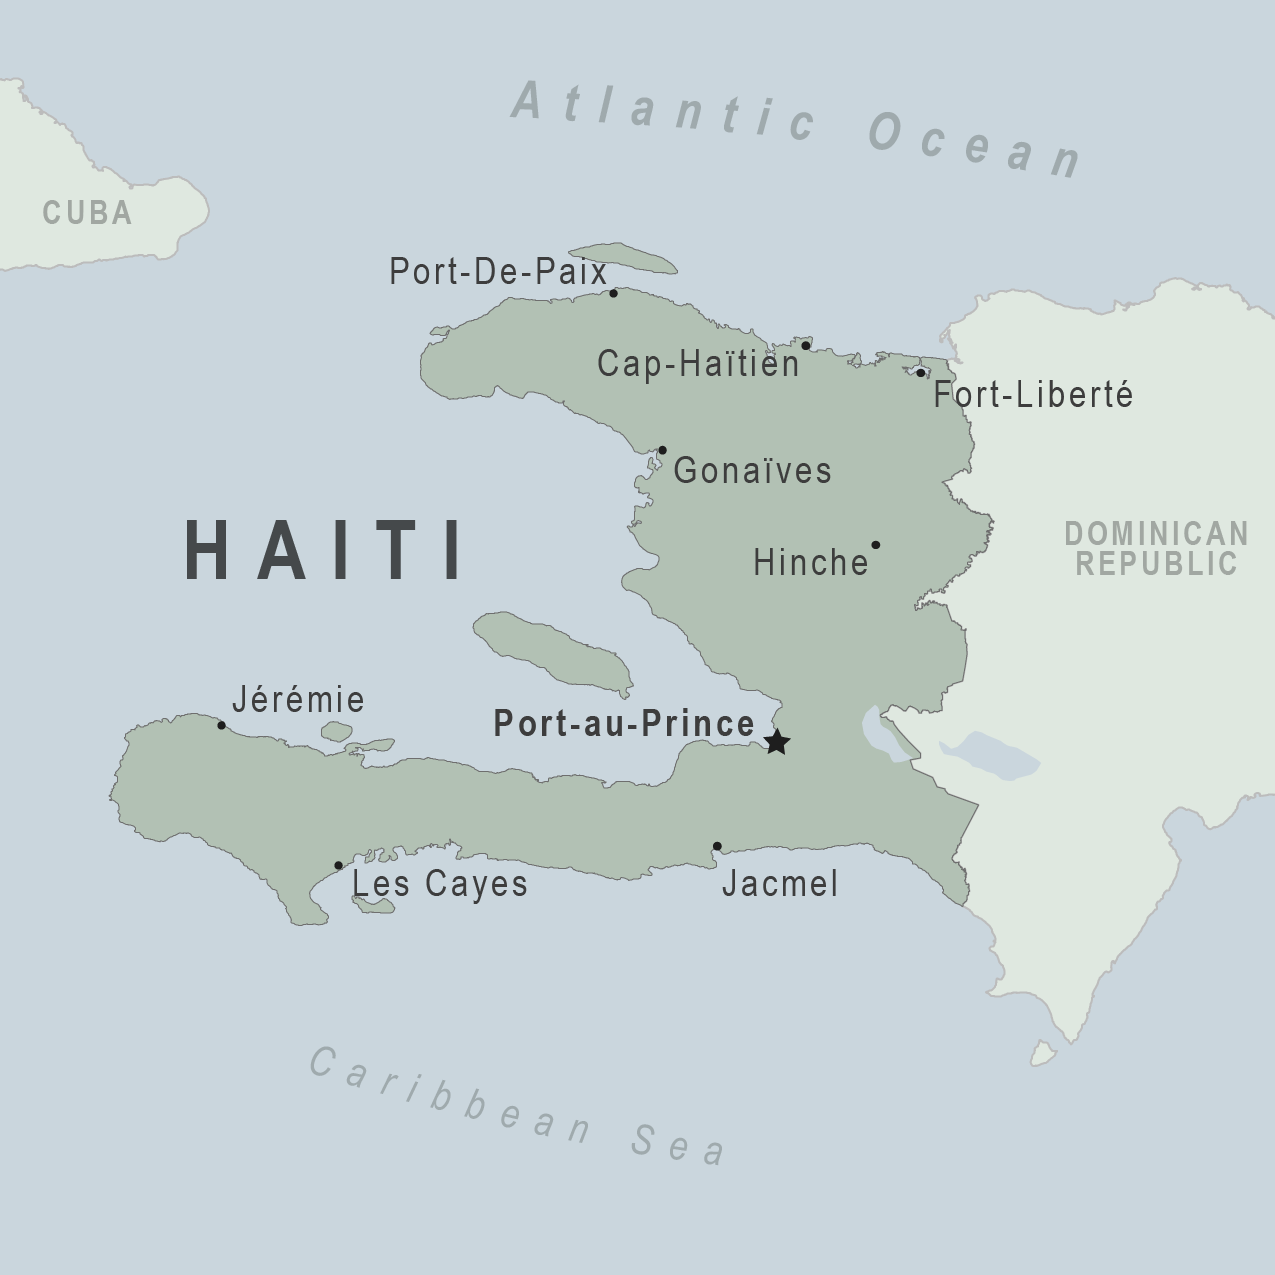
\includegraphics[width=1\textwidth]{images/Contexte/map-haiti.png}
        \caption{Cartographie d'Haïti}
    \end{figure}